\chapter{Aplicação Proposta}
\label{chapter:app_proposta}


As aplicações de geolocalização atualmente disponíveis na maioria dos dispositivos utilizam mapas ou imagens
provenientes de satélites. Para o usuário, esse tipo de visualização pode não ser satisfatória, pois não revela
informações e detalhes da realidade à sua volta.

Para o usuário de uma aplicação de geolocalização, o programa deveria não apenas exibir uma visão geral do terreno,
por meio de mapas ou imagens de satélite, mas, também, permitir visualizar informações de pontos de interesse ao
seu redor, bem como sua distância até eles, por meio de uma visualização do ambiente a partir de sua perspectiva. 
Ou seja, na tela de seu dispositivo, deveria ser exibida a imagem que ele vê com os próprios olhos, o que tornaria a
aplicação muito mais interativa.



Como trabalho prático, de implementação, foi desenvolvido um aplicativo
para dispositivos móveis usando técnicas de Realidade Aumentada para criar uma ferramenta
que facilite a localização de usuários nos campi da Universidade Federal do Paraná. 

O aplicativo fornece uma visualização de mapa, onde estão listados pontos de interesse
para alunos e funcionários da Universidade Federal do Paraná. Esse mapa será obtido por meio das
\glspl{API} oficiais do sistema operacional do dispositivo em que
o sistema é executado. As localizações de cada ponto de interesse são exibidas conforme
suas coordenadas geográficas (latitude e longitude).

Há outro modo de visualização, o qual envolve a Realidade Aumentada. Nesse modo,
a imagem da câmera é exibida na tela do dispositivo, com
os pontos de interesse próximos demarcados nela, de forma que, ao mover o aparelho
lateralmente, as referências aos pontos de interesse também se movem na tela, orientando o
usuário a como chegar a eles e informando qual é a distância até eles. Conforme o usuário
se move no espaço, atualizam-se os dados exibidos na tela. Isso inclui recalcular a
distância até os pontos de interesses, além de atualizar a visualização com essas novas
informações.

Foram mapeados alguns locais de interesse do campus Centro Politécnico,
da Universidade Federal do Paraná, em Curitiba, fixando pontos de referência, como, por exemplo:

\begin{itemize}
    \item Secretarias de cursos
    \item Coordenações de cursos
    \item Departamentos
    \item Restaurantes Universitários
    \item Centros Acadêmicos
    \item Lanchonetes
    \item Caixas Eletrônicos
    \item Bibliotecas
    \item Blocos de salas de aula
    \item Pontos de ônibus próximos aos campi
    \item Pontos do ônibus InterCampi
\end{itemize}



Há, também, uma interface de configurações, onde cada usuário pode adicionar, editar e remover
novos pontos de interesse que sejam úteis para ele.


A visualização em formato de mapas destaca os pontos de interesse por meio de alfinetes vermelhos,
que, quanto tocados, exibem o nome da localização. A Figura \ref{fig:pins-maps} ilustra a visualização de alguns
pontos do Centro Politécnico da Universidade Federal do Paraná, na visualização de mapas.

\begin{figure}[h!]
    \centering
    \caption{Exibição de locais na visualização de Mapas do Aplicativo Desenvolvido}
    \label{fig:pins-maps}
    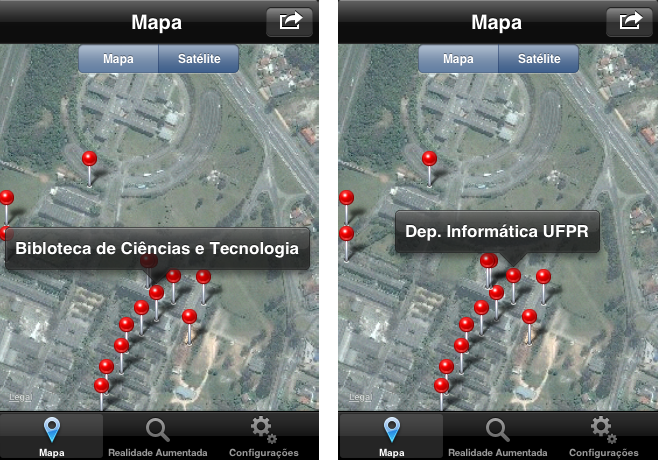
\includegraphics[width=14cm]{resources/App_Maps_Screenshots/mapa-pins.png}
\end{figure}

No canto superior esquerdo, há um botão que abre um menu de ações, ilustrado na 
Figura \ref{fig:maps-action-menu}. Por meio desse menu, é possível salvar a
atual localização do usuário, para criar um novo local de interesse; também é
possível centralizar o mapa na localização atual do usuário; além disso, também
é possível abrir uma lista dos locais salvos, para que o usuário selecione o ponto
que deseja visualizar no mapa.

\begin{figure}[h!]
    \centering
    \caption{Menu de ações relacionadas aos mapas no aplicativo desenvolvido}
    \label{fig:maps-action-menu}
    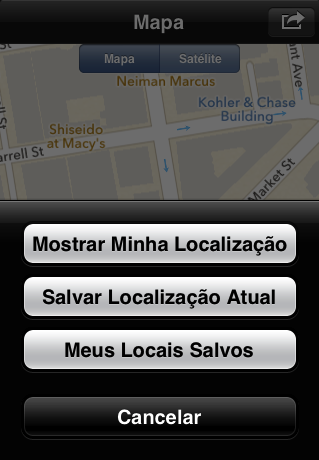
\includegraphics[width=10cm]{resources/App_Maps_Screenshots/action-menu.png}
\end{figure}



A Figura \ref{fig:App-AR-Screenshot} exibe um exemplo da visualização em Realidade Aumentada
do aplicativo.

\begin{figure}[h!]
    \centering
    \caption{Visualização em Realidade Aumentada do aplicativo proposto}
    \label{fig:App-AR-Screenshot}
    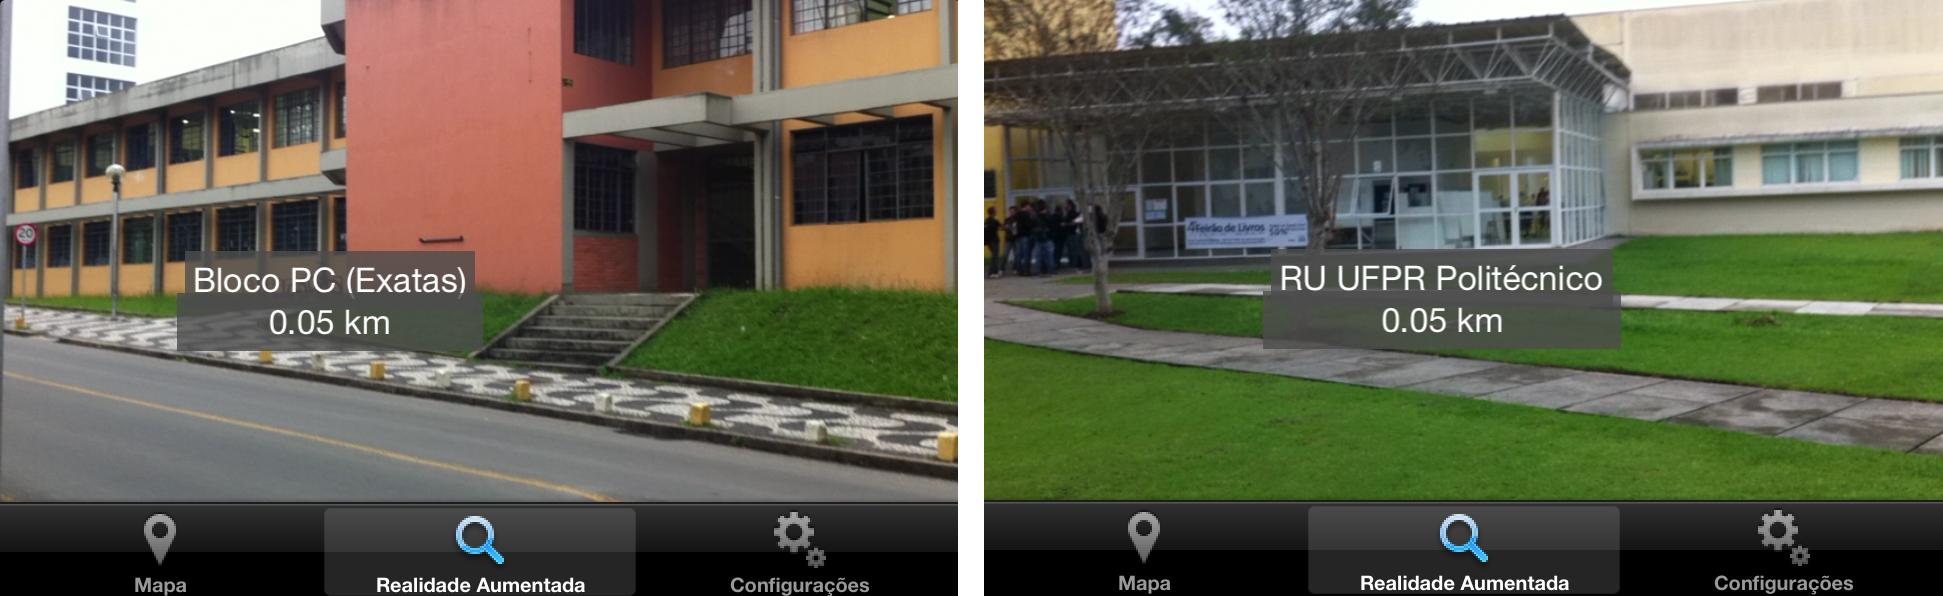
\includegraphics[width=17cm]{resources/App_AR_Screenshots/AR-sceenshot.png}
\end{figure}



\section{Detalhes da Implementação}


Como ferramenta base para o desenvolvimento, foi usado o \textbf{iPhone-AR-Toolkit}
\footnote{\href{https://github.com/nielswh/iPhone-AR-Toolkit}{https://github.com/nielswh/iPhone-AR-Toolkit}},
que também foi utilizado por William Chang e Qing Tan em \cite{MOOAR_Study}.
Essa ferramenta utiliza o conceito de \textit{``Multi-Object Oriented Augmented Reality''} (MOOAR), o qual 
foi descrito com mais detalhes na Seção \ref{sec:trab_relacionados} deste texto.

A aplicação utiliza técnicas de \textit{Tracking} e \textit{Registration} para utilização em ambientes 
externos (\textit{outdoor}). A detecção da posição e da orientação da câmera do dispositivo usado pelo 
usuário é feita utilizando-se
\gls{GPS}, acelerômetro e giroscópio. Ou seja, são utilizados \textit{Tracking} baseado em sensores 
(\textit{Sensor-Based Tracking}) e \textit{Registration} baseado em rastreamento 
(\textit{Tracking-based Registration}).


O dispositivo utilizado para testar a aplicação foi um Apple iPhone 4. A escolha foi feita devido à capacidade deste 
equipamento de obter dados de localização global (\gls{GPS}), além de possuir acelerômetro e giroscópio, permitindo
obter informações precisas da posição e da orientação do aparelho (\gls{6DOF}).


Com base na localização do usuário, a aplicação busca locais próximos conhecidos, cadastrados em uma base de dados
local do dispositivo, onde há, dentre outras informações, suas latitude e a longitude. Conforme a posição e a
orientação do usuário no espaço tridimensional, são exibidas imagens na tela do dispositivo, mostrando ao usuário
em qual direção cada local está e qual a distância até ele. A medida que o usuário se move, esses dados são atualizados,
de forma a funcionar como um guia para quem não conhece a região ou procura por um local ainda desconhecido para ele.

A linguagem utilizada foi a Objective-C, linguagem padrão da \gls{SDK} do iOS, sistema operacional para dispositivos 
móveis da Apple.


\subsection{Base de dados}

Para aplicações em dispositivos móveis de baixo consumo, costuma-se usar o SQLite
\footnote{\href{http://www.sqlite.org}{http://www.sqlite.org}} como \gls{SGBD}, 
por utilizar poucos recursos de armazenamento e processamento. A aplicação proposta
também utiliza o SQLite, por meio do \textit{Core Data}, uma interface fornecida 
pela Apple para acesso a bases de dados.

A estrutura do banco de dados é formada por apenas uma tabela, a qual armazena as
seguintes informações sobre os pontos de interesse: nome (uma \textit{string}), 
latitude (um número no formato \textit{float}) e longitude (um número no 
formato \textit{float}). A Figura \ref{fig:modelo_dados} mostra o modelo de dados 
da aplicação.


\begin{figure}[h!]
    \centering
    \caption{Modelo de dados da aplicação proposta}
    \label{fig:modelo_dados}
    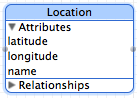
\includegraphics[width=4cm]{resources/App_Source_Code/db-scheme.png}
\end{figure}



O aplicativo é iniciado com uma base de dados inicial, com os principais pontos de interesse do campus Centro Politécnico
da Universidade Federal do Paraná. Essas informações iniciais ficam salvas em um arquivo \gls{XML}, formatado conforme
o padrão PLIST\footnote{\href{http://filext.com/file-extension/PLIST}{http://filext.com/file-extension/PLIST}} 
(\textit{Property List}), com os dados dos pontos de interesse, como nome, latitude e longitude. A Figura 
\ref{fig:plist-file} mostra como é a estrutura desse arquivo. O Algoritmo \ref{alg:load-plist-file} exibe o
trecho de código que carrega os dados desse arquivo e os salva na base de dados.


\begin{figure}[h!]
    \centering
    \caption{Arquivo XML com os dados iniciais da base de dados da aplicação proposta}
    \label{fig:plist-file}
    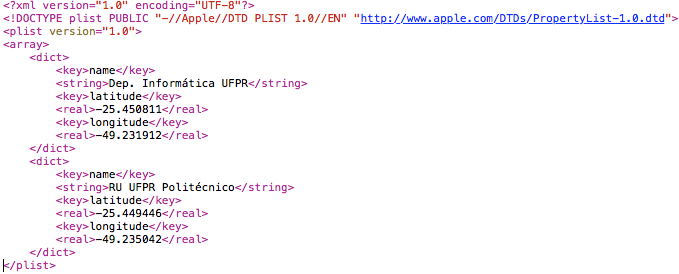
\includegraphics[width=17cm]{resources/App_Source_Code/plist-file.png}
\end{figure}



\begin{sourcecode}{alg:load-plist-file}{Trecho de código que carrega os dados do Arquivo XML para o SQLite}
- (void) loadInitialCoreDataInfo
{
    // array com os arquivos PLIST que devem ser carregados no Core Data
    NSArray *plistFiles = @[@{@"basename" : @"places_politecnico", @"extension" : @"plist"}];

    for ( NSDictionary *plistDict in plistFiles )
    {
        NSString *path = [[NSBundle mainBundle] pathForResource:plistDict[@"basename"] ofType:plistDict[@"extension"]];

        NSFileManager *fileManager = [NSFileManager defaultManager];

        if ( ! [fileManager fileExistsAtPath:path] )
        {
            NSLog(@"Arquivo '%@' nao existe", path);
            continue;
        }

        NSArray *locations = [NSArray arrayWithContentsOfFile:path];

        for ( NSDictionary *locationDict in locations )
        {
            NSString *name = locationDict[@"name"];
            NSNumber *latitude = locationDict[@"latitude"];
            NSNumber *longitude = locationDict[@"longitude"];

            [Location saveLocation:name latitude:[latitude floatValue] longitude:[longitude floatValue]];
        }
    }
}
\end{sourcecode}


\subsection{Integração com o iPhone-AR-Toolkit}

O \textit{iPhone-AR-Toolkit} não é uma biblioteca, nem um \textit{framework}. Ele é um
projeto ainda em desenvolvimento, com alguns recursos não muito aprimorado até o momento. Ou seja,
não basta apenas importar os arquivos e chamar um método específico. Porém, sua integração
com outras aplicações não é muito complexa. Seguindo o padrão da aplicação de demonstração, 
disponibilizada também no \textit{GitHub}, com algumas modificações e adaptações, é 
possível ter uma aplicação funcional.

A \gls{SDK} do iOS utiliza o padrão de projeto \textit{Delegation}. Esse é um padrão
utilizado na Programação Orientada a Objetos onde um objeto A, em vez de executar uma
determinada tarefa, delega-a para um objeto B. O \textit{iPhone-AR-Toolkit} também
utiliza esse padrão de projeto em diversas partes de seu código.


O Algoritmo \ref{alg:display_ar} ilustra o método responsável por carregar a \textit{view}
da Realidade Aumentada. O objeto \texttt{arc} é uma instância da classe 
\texttt{AugmentedRealityController}, que é responsável pelas operações relacionadas à
Realidade Aumentada. O objeto \texttt{arView} é uma instância da classe \texttt{UIView},
padrão da \gls{SDK} do iOS. Durante a instanciação de \texttt{arc}, na linha 5, é definido o seu
\textit{delegate} para \textit{self}, ou seja, o próprio objeto. Nesse ponto é usado o 
padrão \textit{Delegation}, quando a classe atual é responsável por executar tarefas da
\texttt{AugmentedRealityController}.


\begin{sourcecode}{alg:display_ar}{Método responsável pelo carregamento da \textit{view} de Realidade Aumentada}
- (void) displayAR
{
    if ([ARKit deviceSupportsAR])
    {
        arc = [[AugmentedRealityController alloc] initWithView:[self arView] parentViewController:self withDelgate:self];

        [self populateGeoLocations];
    }
    else
    {
        [self notSupportView];
    }
}
\end{sourcecode}


Antes de habilitar a funcionalidade de Realidade Aumentada, é necessário verificar se o dispositivo
suportará esse recurso. Para isso, o equipamento deve possuir câmera, além de sensor de \gls{GPS},
para detecção da localização do usuário. O Algoritmo \ref{alg:device-supports-ar} mostra o método
responsável por essas verificações. Para detecção da presença de câmera, usam-se algumas classes e
métodos do \textit{framework} \texttt{AVFoundation}, nativo do iOS. Para verificação da presença de
\gls{GPS} e suporte a localização, usa-se o método \texttt{headingAvailable])}, da classe 
\texttt{CLLocationManager}, presente no \textit{framework} \texttt{CoreLocation}, 
também nativo do iOS.

\begin{sourcecode}{alg:device-supports-ar}{Método para verificar se o dispositivo suporta o recurso de Realidade Aumentada}
+(BOOL)deviceSupportsAR
{
    // verifica o suporte a captura de video
    NSArray *devices = [AVCaptureDevice devices];

    BOOL suportsVideo = NO;

    if (devices != nil && [devices count] > 0) 
    {
        for (AVCaptureDevice *device in devices) 
        {
            if ([device hasMediaType:AVMediaTypeVideo]) 
            {
                suportsVideo = YES;
                break;
            }
        }
    }

    if (!suportsVideo)
    {
        return NO;
    }
    
    // verifica suporte a GPS
	if ( [CLLocationManager headingAvailable])
	{
		return NO;
	}

	return YES;
}
\end{sourcecode}



O método \texttt{populateGeoLocations} é responsável por buscar na base de dados as informações
acerca dos pontos de interesse, como nome, latitude e longitude. Esse método também cria as 
\textit{views} que servirão de marcadores, as quais serão sobrepostas às imagens da câmera, 
conforme a localização e a direção do dispositivo. O Algoritmo \ref{alg:populate-geolocations}
exibe a implementação desse método.



\begin{sourcecode}{alg:populate-geolocations}{Método responsável pelo carregamento das localizações e criação dos marcadores na tela do dispositivo}
- (void) populateGeoLocations
{
    GEOLocations* locations = [[GEOLocations alloc] initWithDelegate:self];

    if ([[locations returnLocations] count] > 0)
    {
        for (ARGeoCoordinate *coordinate in [locations returnLocations])
        {

            MarkerView *cv = [[MarkerView alloc] initForCoordinate:coordinate withDelgate:self] ;
            [coordinate setDisplayView:cv];

            [arc addCoordinate:coordinate];
        }
    }
}
\end{sourcecode}



O método \texttt{initWithView:parentViewController:withDelgate:}, utilizado na linha 5 do
Algoritmo \ref{alg:display_ar}, é responsável por inicializar o objeto 
\texttt{AugmentedRealityController}, subclasse de \texttt{NSObject}, a qual é a classe base
de todos os objetos no Objective-C. Além de definir algumas propriedades internas do objeto, 
este método instancia os objetos responsáveis por carregar as imagens provenientes da câmera
do dispositivo. Note que esse procedimento é realizado dentro de um \texttt{if}, na linha 22, o qual verifica
se a aplicação não estará sendo executada no \textit{iPhone Simulator}, simulador do iPhone disponibilizado
pela Apple juntamente com a \gls{SDK} do iOS. Como o simulador não possui câmera, essa verificação é
necessária, para evitar erros durante a execução. O método também adiciona, na linha 61, um método responsável por
redesenhar a \textit{view} se a orientação do dispositivo mudar (vertical ou horizontal). Para isso, é usada
a class \texttt{NSNotificationCenter}, do iOS, que registra notificações que ficam disponíveis durante todo o 
tempo de vida da aplicação.


\begin{sourcecode}{alg:initAR}{Método responsável por instanciar a \textit{view} de Realidade Aumentada e iniciar os recursos de câmera e GPS}
- (id)initWithView:(UIView*)arView parentViewController:(UIViewController*)parentVC withDelgate:(id<ARDelegate>) aDelegate
{    
    if (!(self = [super init]))
		return nil;

    [self setParentViewController:parentVC];
    [self setDelegate:aDelegate];

    latestHeading   = HEADING_NOT_SET;
    prevHeading     = HEADING_NOT_SET;

    [self setMaximumScaleDistance: 0.0];
	[self setMinimumScaleFactor: SCALE_FACTOR];
	[self setScaleViewsBasedOnDistance: NO];
	[self setRotateViewsBasedOnPerspective: NO];
	[self setMaximumRotationAngle: M_PI / 6.0];
    [self setCoordinates:[NSMutableArray array]];
    [self currentDeviceOrientation];

	degreeRange = [arView frame].size.width / ADJUST_BY;

#if !TARGET_IPHONE_SIMULATOR

    NSError *error = nil;
    AVCaptureSession *avCaptureSession = [[AVCaptureSession alloc] init];
    AVCaptureDevice *videoCaptureDevice = [AVCaptureDevice defaultDeviceWithMediaType:AVMediaTypeVideo];
    AVCaptureDeviceInput *videoInput = [AVCaptureDeviceInput deviceInputWithDevice:videoCaptureDevice error:&error];

    if (videoInput) {
        [avCaptureSession addInput:videoInput];
    }
    else {
        // Handle the failure.
    }

    AVCaptureVideoPreviewLayer *newCaptureVideoPreviewLayer = [[AVCaptureVideoPreviewLayer alloc] initWithSession:avCaptureSession];

    [[arView layer] setMasksToBounds:YES];
    [newCaptureVideoPreviewLayer setFrame:[arView bounds]];
    [newCaptureVideoPreviewLayer setVideoGravity:AVLayerVideoGravityResizeAspectFill];

    if ([[newCaptureVideoPreviewLayer connection] isVideoOrientationSupported])
        [[newCaptureVideoPreviewLayer connection] setVideoOrientation:cameraOrientation];

    [newCaptureVideoPreviewLayer setVideoGravity:AVLayerVideoGravityResizeAspectFill];
    [[arView layer] insertSublayer:newCaptureVideoPreviewLayer below:[[[arView layer] sublayers] objectAtIndex:0]];

    [self setPreviewLayer:newCaptureVideoPreviewLayer];

    [avCaptureSession setSessionPreset:AVCaptureSessionPresetHigh];
    [avCaptureSession startRunning];

    [self setCaptureSession:avCaptureSession];  

#endif

    CLLocation *newCenter = [[CLLocation alloc] init];

	[self setCenterLocation: newCenter];

	[[NSNotificationCenter defaultCenter] 
	 addObserver:self 
	 selector:@selector(deviceOrientationDidChange:)
     name:UIDeviceOrientationDidChangeNotification 
     object:nil];

	[self startListening];
    [self setDisplayView:arView];

  	return self;
}
\end{sourcecode}


O método \texttt{startListening}, na linha 66 do Algoritmo \ref{alg:initAR},
é encarregado de iniciar a atualização da localização, conforme o usuário
se move no espaço, além de habilitar o uso do acelerômetro, para detecção
da orientação do dispositivo. O Algoritmo \ref{alg:startListening} mostra a 
implementação desse método.

\begin{sourcecode}{alg:startListening}{Implementação do método \texttt{startListening}}
- (void)startListening
{
	// start our heading readings and our accelerometer readings.
	if (![self locationManager]) {
		CLLocationManager *newLocationManager = [[CLLocationManager alloc] init];

        [newLocationManager setHeadingFilter: HEADING_FILTER];
        [newLocationManager setDistanceFilter:DISTANCE_FILTER];
		[newLocationManager setDesiredAccuracy: kCLLocationAccuracyNearestTenMeters];
		[newLocationManager startUpdatingHeading];
		[newLocationManager startUpdatingLocation];
		[newLocationManager setDelegate: self];

        [self setLocationManager: newLocationManager];
	}

	if (![self accelerometerManager]) {
		[self setAccelerometerManager: [UIAccelerometer sharedAccelerometer]];
		[[self accelerometerManager] setUpdateInterval: INTERVAL_UPDATE];
		[[self accelerometerManager] setDelegate: self];
	}

	if (![self centerCoordinate]) 
		[self setCenterCoordinate:[ARCoordinate coordinateWithRadialDistance:1.0 inclination:0 azimuth:0]];
}
\end{sourcecode}


O método \texttt{updateLocations}, cuja implementação está exibida no Algoritmo
\ref{alg:updateLocations}, é o responsável por alterar os marcadores de pontos de
interesse exibidos na tela do dispositivo, conforme o usuário se move.

\begin{sourcecode}{alg:updateLocations}{Implementação do método \texttt{updateLocations}}
- (void)updateLocations
{
	for (ARGeoCoordinate *item in [self coordinates]) {

        UIView *markerView = [item displayView];

		if ([self shouldDisplayCoordinate:item]) {

            CGPoint loc = [self pointForCoordinate:item];
            CGFloat scaleFactor = SCALE_FACTOR;

			if ([self scaleViewsBasedOnDistance]) 
				scaleFactor = scaleFactor - [self minimumScaleFactor]*([item radialDistance] / [self maximumScaleDistance]);

			float width	 = [markerView bounds].size.width  * scaleFactor;
			float height = [markerView bounds].size.height * scaleFactor;

			[markerView setFrame:CGRectMake(loc.x - width / 2.0, loc.y, width, height)];
            [markerView setNeedsDisplay];

			CATransform3D transform = CATransform3DIdentity;

			// Set the scale if it needs it. Scale the perspective transform if we have one.
			if ([self scaleViewsBasedOnDistance]) 
				transform = CATransform3DScale(transform, scaleFactor, scaleFactor, scaleFactor);

			if ([self rotateViewsBasedOnPerspective]) {
				transform.m34 = 1.0 / 300.0;
			}
			[[markerView layer] setTransform:transform];

			//if marker is not already set then insert it
			if (!([markerView superview])) {
				[[self displayView] insertSubview:markerView atIndex:1];
			}
		} 
		else 
            if ([markerView superview])
                [markerView removeFromSuperview];

	}
}
\end{sourcecode}


O aplicativo foi desenvolvido para iOS 6.0 ou superior, com suporte a iPhone e iPad. O 
código-fonte está disponível em \href{https://github.com/beraldo/TG}{https://github.com/beraldo/TG}.





